\documentclass[11pt]{beamer}
\usetheme{Dresden}
\usepackage[utf8]{inputenc}
\usepackage[ngerman]{babel}
\usepackage[T1]{fontenc}
\usepackage{amsmath}
\usepackage{amsfonts}
\usepackage{amssymb}
\usepackage{pifont}
\usepackage{color, colortbl}
\newcommand{\cmark}{\ding{51}}
\newcommand{\xmark}{\ding{55}}
\usepackage{fontawesome}

\usepackage{adjustbox}

% \usepackage{emoji}


\usepackage[backend=biber,
style=alphabetic,
]{biblatex}



\usecolortheme{beaver}


\title[Anwendungsfach / Nebenfach: Maschinenbau] % (optional, only for long titles)
{Maschinenbau}
\author {Pina \faHandPeaceO}


\date[WiSe2021] % (optional)
{Anwendungsfach / Nebenfach}
\subject{Computer Science}

\beamertemplatenavigationsymbolsempty


\begin{document}



%------------------------------------------------------


\begin{frame}
	\titlepage
\end{frame}





%------------------------------------------------------







\begin{frame}{Nebenfach und Anwendungsfach}


\begin{columns}[T] % align columns
\begin{column}{.48\textwidth}
\color{red}

Kerninformatik: \\
\begin{itemize}
\item Nebenfach mit 20 CP
\end{itemize}


\end{column}%
\hfill%
\begin{column}{.48\textwidth}
\color{blue}


Angewandte Informatik: \\
\begin{itemize}
\item Anwendungsfach mit 36 CP
\end{itemize}


\end{column}%
\end{columns}
\end{frame}




%------------------------------------------------------




\begin{frame}{Pflichtmodule}




\begin{columns}[T] % align columns
\begin{column}{.48\textwidth}
\color{red}

Kerninformatik: \vspace*{2em}
\color{black}
\adjustbox{max width=\textwidth}{%
\begin{tabular}{l l}
& \\
\textbf{Fertigungslehre} & 3CP \\
\textbf{Technisches Zeichnen} & 3CP \\
\textbf{Maschinenelemente} & 4CP \\
Wahlmodul & 5CP \\
Wahlmodul & 5 CP \\

\end{tabular}}


\end{column}%
\hfill%
\begin{column}{.48\textwidth}
\color{blue}


Angewandte Informatik: \vspace*{2em}
\color{black}
\adjustbox{max width=\textwidth}{%
\begin{tabular}{l l}
& \\
\textbf{Fertigungslehre} & 3CP \\
\textbf{Technisches Zeichnen} & 3CP \\
\textbf{Maschinenelemente I} & 4CP \\
Maschinenelemente II & 4CP \\
Technische Mechanik I & 5CP \\
Werkstofftechnik & 5CP \\
Elektrotechnik & 4CP \\
2 Wahlmodule & 8CP
 

\end{tabular} }


\end{column}%
\end{columns}



\end{frame}





%------------------------------------------------------






\begin{frame}{Fertigungslehre}

\begin{columns}[T] % align columns
\begin{column}{.5\textwidth}

\textbf{Spanende Fertigungslehre:} \\
\begin{itemize}
\item z.B. Material bohren, sägen, schleifen
\end{itemize}


\end{column}%
\hfill%
\begin{column}{.5\textwidth}


\textbf{Umformende Fertigungslehre:} \\
\begin{itemize}
\item z.B. Material biegen, walzen, gießen etc.
\end{itemize}


\end{column}%
\end{columns}

\begin{itemize}
\item[]
\item[]
\item verschiedene Konzepte und Verfahren kennen und unterscheiden
\end{itemize}
	
\end{frame}







%------------------------------------------------------







\begin{frame}{Technisches Zeichnen - 3-Tafel-Projektion}

\begin{center}
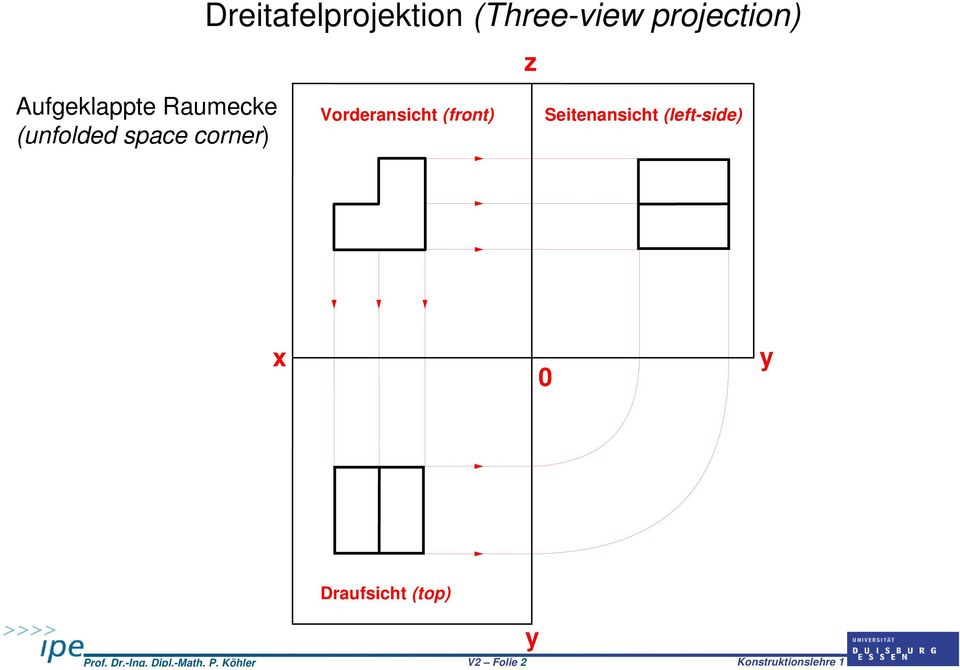
\includegraphics[scale=1]{page_2.jpg}
\end{center}

	
\end{frame}







%------------------------------------------------------





\begin{frame}{Technisches Zeichnen - isometrische/dimetrische Ansicht}

\begin{center}
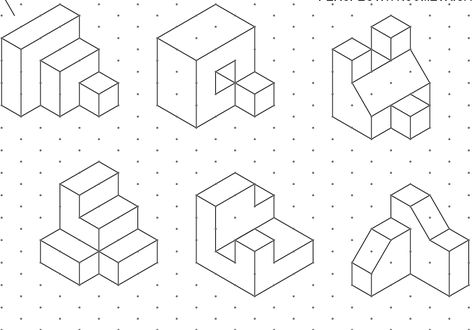
\includegraphics[scale=0.5]{iso.jpg}
\end{center}

\begin{itemize}
\item isometrische Ansicht
\end{itemize}
	
\end{frame}







%------------------------------------------------------





\begin{frame}{Technisches Zeichnen - Wellenbemaßung}

\begin{center}
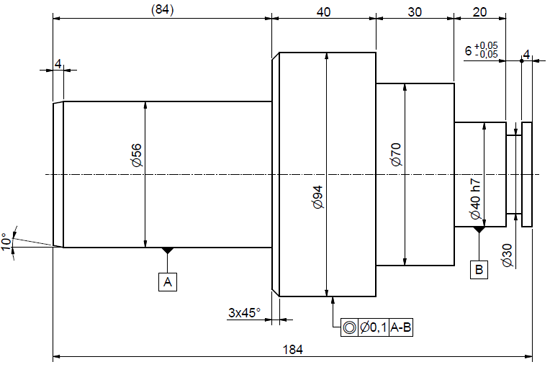
\includegraphics[scale=0.5]{welle.png}
\end{center}

	
\end{frame}







%------------------------------------------------------




\begin{frame}{Maschinenelemente}
	
\begin{itemize}
\item Werkstoffe und Werkstoffeigenschaften
\item Schweißverfahren
\item Federungen
\item Achsen und Wellen
\item Dichtungen
\end{itemize}
	
	
\end{frame}





\begin{frame}{Fragen}
	
\begin{itemize}
\item Fragen?
\end{itemize}
	
	
\end{frame}









\end{document}